El modelado tridimensional de los componentes estructurales del sistema se realizó mediante software CAD, permitiendo la visualización detallada de cada elemento, la verificación de interferencias geométricas y el análisis de esfuerzos mediante simulación por elementos finitos. En esta sección se presentan los tres soportes estructurales principales fabricados mediante impresión 3D, junto con el brazo robótico y su efector final. Se incluye además el análisis de esfuerzos del soporte superior, que constituye el elemento más crítico desde el punto de vista de cargas estructurales.

\subsubsection{Soporte Superior}

El soporte superior constituye el elemento estructural de mayor criticidad en el sistema, ya que soporta la totalidad de las cargas verticales (varillas, brazo, carga) y actúa como interfaz mecánica entre los subsistemas de movimiento horizontal y vertical. Su diseño integra múltiples funciones: acoplamiento a los carros deslizantes del perfil horizontal, fijación de los extremos superiores de las tres varillas verticales (una roscada y dos lisas), y montaje del motor del eje vertical.

La Figura \ref{fig:SuperiorReal_simplificado_vista} muestra la geometría general del soporte superior.

Para el análisis por elementos finitos se consideró la condición de carga más desfavorable: sistema completamente extendido con carga máxima en el extremo del brazo. La carga total aplicada sobre el soporte superior se compone de:

\begin{itemize}
    \item Peso de las tres varillas verticales (dos lisas de acero + una roscada): $\approx$ 3.8 kg
    \item Peso del soporte medio con brazo y cámara: $\approx$ 1.5 kg
    \item Peso del motor vertical: $\approx$ 2.2 kg
    \item Carga útil (lechuga) en extremo del brazo: $\approx$ 0.4 kg
    \item Peso propio del soporte superior: $\approx$ 1.1 kg
\end{itemize}

La carga total considerada para el análisis fue de 9 kg ($\approx$ 88 N), aplicada como fuerzas distribuidas sobre las superficies de contacto con las varillas y reacciones de apoyo en las zonas de montaje a los carros, como se muestra en la Figura \ref{fig:SuperiorReal_simplificado_fuerzas_app}.

\begin{figure}[H]
    \centering
    \begin{subfigure}{0.35\textwidth}
        \centering
        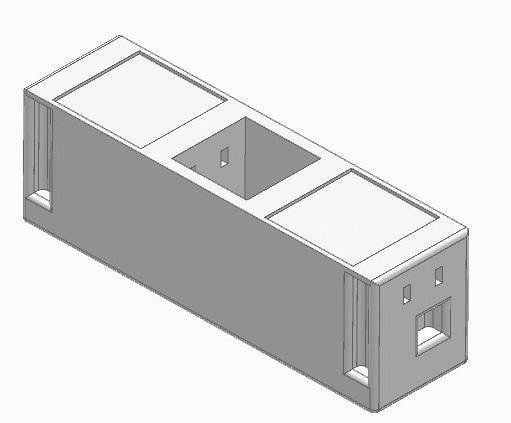
\includegraphics[width=0.7\textwidth]{img/SuperiorReal_simplificado_vista.jpg}
        \caption{Vista del soporte superior mostrando la configuración estructural, alojamientos de varillas y zonas de montaje.}
        \label{fig:SuperiorReal_simplificado_vista}
    \end{subfigure}
    \hspace{0.5cm}
    \begin{subfigure}{0.35\textwidth}
        \centering
        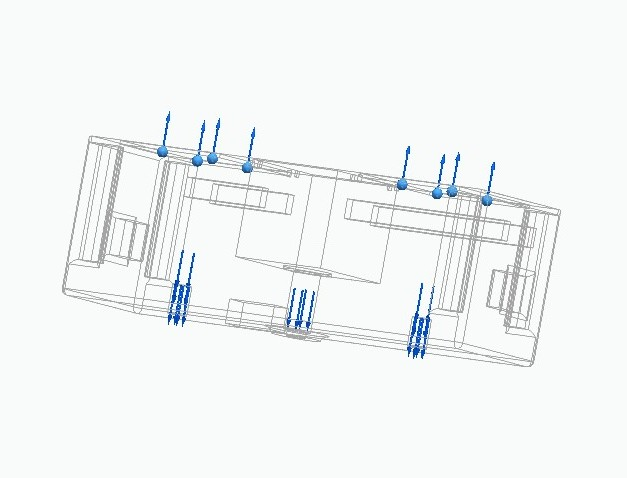
\includegraphics[width=0.7\textwidth]{img/SuperiorReal_simplificado_fuerzas_app.jpg}
        \caption{Distribución de cargas aplicadas sobre el soporte superior.}
        \label{fig:SuperiorReal_simplificado_fuerzas_app}
    \end{subfigure}
    \caption{Soporte superior. Vista y fuerzas aplicadas}
\end{figure}

El análisis de esfuerzos mediante elementos finitos se realizó considerando material PLA con las siguientes propiedades mecánicas:

\begin{itemize}
    \item Módulo de Young: 3500 MPa
    \item Límite de fluencia: 50 MPa
    \item Coeficiente de Poisson: 0.36
\end{itemize}

La Figura \ref{fig:SuperiorReal_simplificado_tensiones} presenta los resultados del análisis, mostrando las deformaciones resultantes. Los resultados indican:

\begin{itemize}
    \item Deformación máxima: $\approx$ 0.15 mm (en zonas de mayor voladizo)
    \item Factor de seguridad: $\frac{50\,\text{MPa}}{2.8\,\text{MPa}} \approx 18$ (ampliamente seguro)
\end{itemize}

\begin{figure}[H]
    \centering
    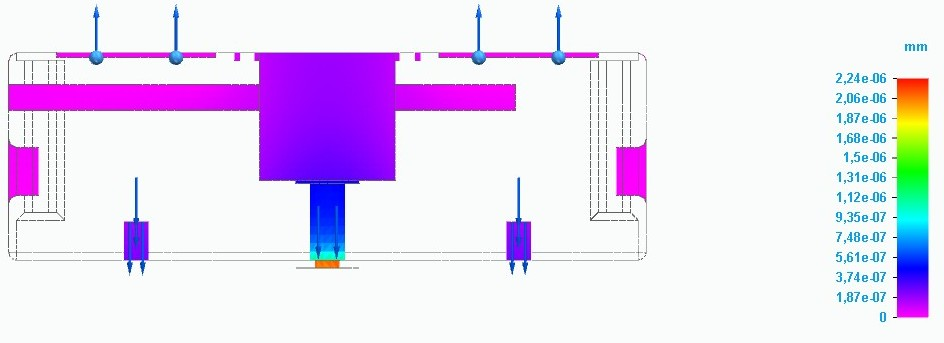
\includegraphics[width=0.6\textwidth]{img/SuperiorReal_simplificado_tensiones.jpg}
    \caption{Distribución de deformaciones en el soporte superior bajo carga máxima. Los valores obtenidos confirman que el diseño es estructuralmente adecuado con amplios márgenes de seguridad.}
    \label{fig:SuperiorReal_simplificado_tensiones}
\end{figure}

Los resultados confirman que el diseño propuesto es estructuralmente robusto, con tensiones muy por debajo del límite de fluencia del material y deformaciones despreciables para los requerimientos operacionales del sistema.

\subsubsection{Soporte Medio}

El soporte medio constituye el elemento móvil del eje vertical, desplazándose a lo largo de las varillas mediante el giro de la varilla roscada. Este componente cumple funciones críticas en el sistema: montaje del brazo robótico serial, fijación de la cámara de visión artificial y mantenimiento del equilibrio dinámico mediante contrapeso.

\begin{itemize}
    \item \textbf{Sistema de guiado:} Incorpora dos rodamientos lineales LM16UU para deslizamiento sobre las varillas lisas de 8 mm, garantizando movimiento suave sin rotaciones indeseadas
    \item \textbf{Tuerca de transmisión:} Alojamiento central para tuerca TR16 que se acopla con la varilla roscada, convirtiendo el movimiento rotacional del motor en desplazamiento lineal
    \item \textbf{Montaje del brazo:} Base horizontal plana con patrón de agujeros para fijación del servomotor base del brazo robótico
    \item \textbf{Montaje de cámara:} Soporte superior para la cámara con ajuste angular para optimización del campo de visión
    \item \textbf{Sistema de balanceo:} Contrapeso en el lado opuesto al brazo para reducir momentos flectores sobre las varillas y mejorar la estabilidad dinámica del sistema
\end{itemize}

\begin{figure}[H]
    \centering
    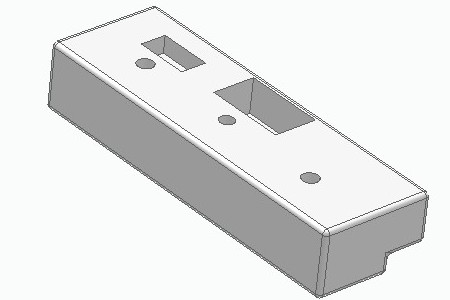
\includegraphics[width=0.5\textwidth]{img/MedioReal_simplificado_vista.jpg}
    \caption{Vista general del soporte medio mostrando el montaje del brazo robótico, alojamiento de la cámara, sistema de guiado lineal y contrapeso de equilibrio.}
    \label{fig:soporte_medio_Real}
\end{figure}

El contrapeso ajustable permite compensar el momento generado por el brazo extendido, reduciendo las cargas laterales sobre las guías lineales y mejorando la precisión de posicionamiento vertical. El diseño modular facilita el reemplazo del brazo o la cámara sin necesidad de rediseñar el soporte completo.

\subsubsection{Soporte Inferior}

El soporte inferior cierra la estructura vertical del sistema, proporcionando la base de fijación para los extremos inferiores de las tres varillas y alojando componentes auxiliares del sistema de control.

\paragraph{Funciones y características}

\begin{itemize}
    \item \textbf{Anclaje de varillas:} Alojamientos pasantes para las dos varillas lisas con fijación mediante tornillos prisioneros, y soporte del extremo libre de la varilla roscada con rodamiento axial
    \item \textbf{Final de carrera inferior:} Montaje del microswitch de límite inferior del eje vertical, con placa de activación mecánica
\end{itemize}

\begin{figure}[H]
    \centering
    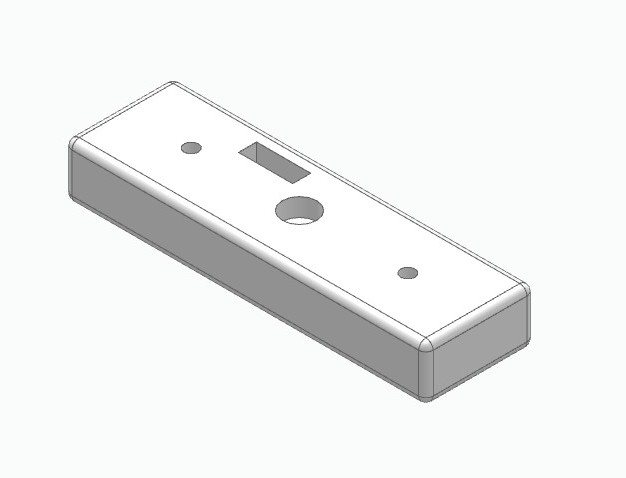
\includegraphics[width=0.5\textwidth]{img/InferiorReal_simplificado_vista.jpg}
    \caption{Soporte inferior mostrando alojamientos de varillas, canales de gestión de cables y montaje del final de carrera.}
    \label{fig:soporte_inferior_real}
\end{figure}

El diseño incorpora tolerancias ajustadas para los alojamientos de las varillas, garantizando la perpendicularidad del eje vertical respecto al plano horizontal de desplazamiento.

\subsubsection{Brazo Robótico Serial}

Se opta por el uso de PLA con fibra de carbono como material estructural proporciona mejor relación rigidez/peso que el PLA estándar, reduciendo las vibraciones residuales al finalizar movimientos rápidos y mejorando la precisión de posicionamiento del efector final.

\begin{figure}[H]
    \centering
    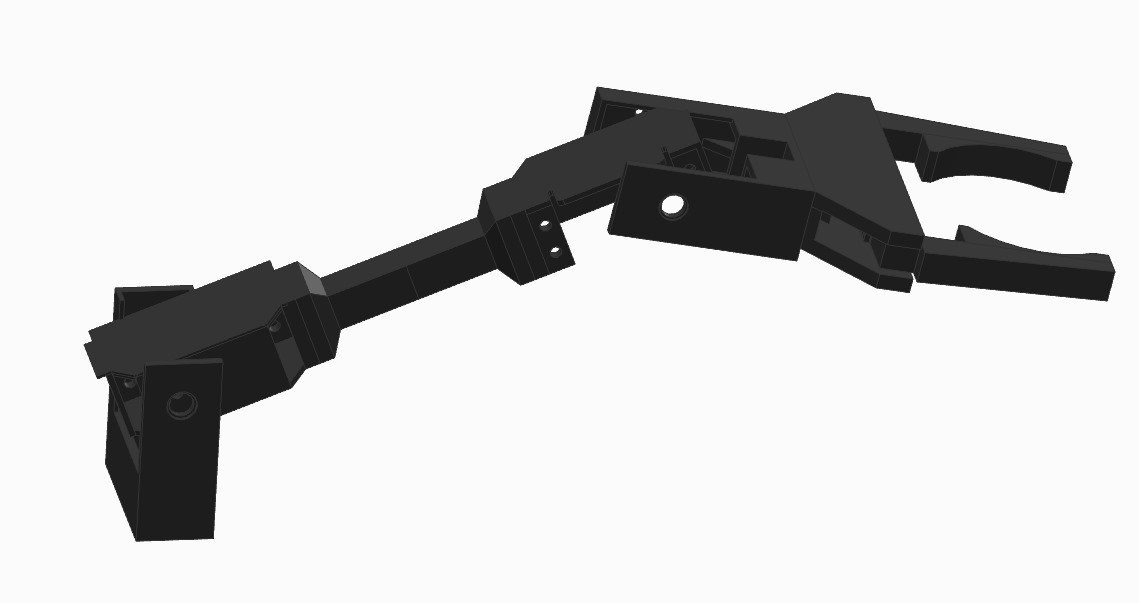
\includegraphics[width=0.5\textwidth]{img/brazo_completo.jpg}
    \caption{Vista completa del brazo robótico de 2 grados de libertad mostrando las dos articulaciones rotacionales y el efector final tipo pinza.}
    \label{fig:brazo_Real}
\end{figure}

\subsubsection{Efector Final - Gripper}

El efector final implementa un mecanismo de pinza paralela actuado mediante transmisión piñón-cremallera, convirtiendo el movimiento rotacional del servomotor en desplazamiento lineal de las mordazas.

\paragraph{Principio de funcionamiento}

\begin{itemize}
    \item \textbf{Transmisión:} Sistema piñón-cremallera con relación 1:1, proporcionando movimiento sincronizado de ambas mordazas hacia el centro
    \item \textbf{Rango de apertura:} 0-80 mm, adecuado para lechugas de tamaño pequeño a grande
    \item \textbf{Fuerza de agarre:} Controlada mediante limitación de corriente del servomotor, evitando daño mecánico a los cultivos
    \item \textbf{Mordazas:} Geometría curva con superficie texturizada para mejorar fricción sin penetrar las hojas
    \item \textbf{Resorte de retorno:} Sistema de resortes internos que garantiza apertura automática ante falla de alimentación
\end{itemize}

\begin{figure}[H]
    \centering
    \begin{subfigure}{0.35\textwidth}
        \centering
        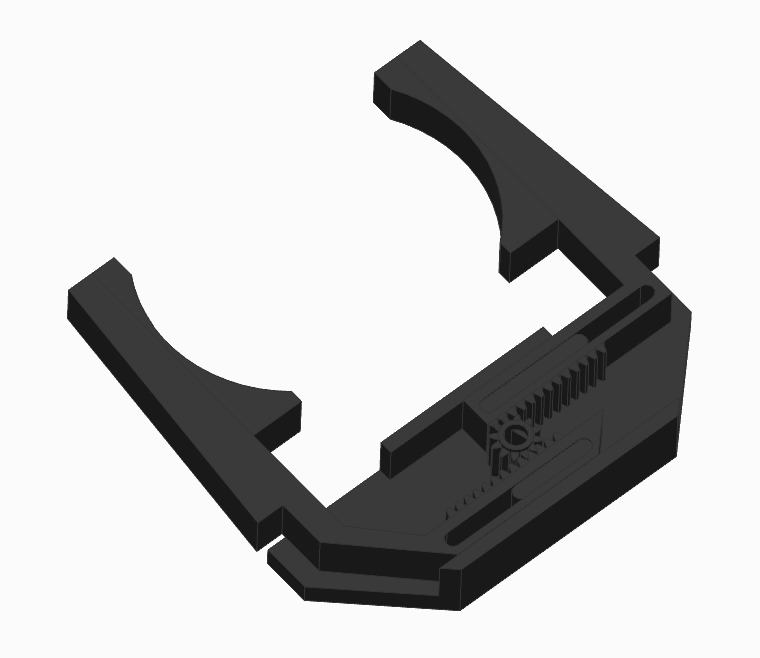
\includegraphics[width=0.7\textwidth]{img/gripper.jpg}
        \caption{Sistema de transmisión piñón-cremallera del gripper mostrando el acoplamiento mecánico entre el servomotor y las mordazas móviles.}
        \label{fig:gripper_Real_transmision}
    \end{subfigure}
    \hspace{0.5cm}
    \begin{subfigure}{0.35\textwidth}
        \centering
        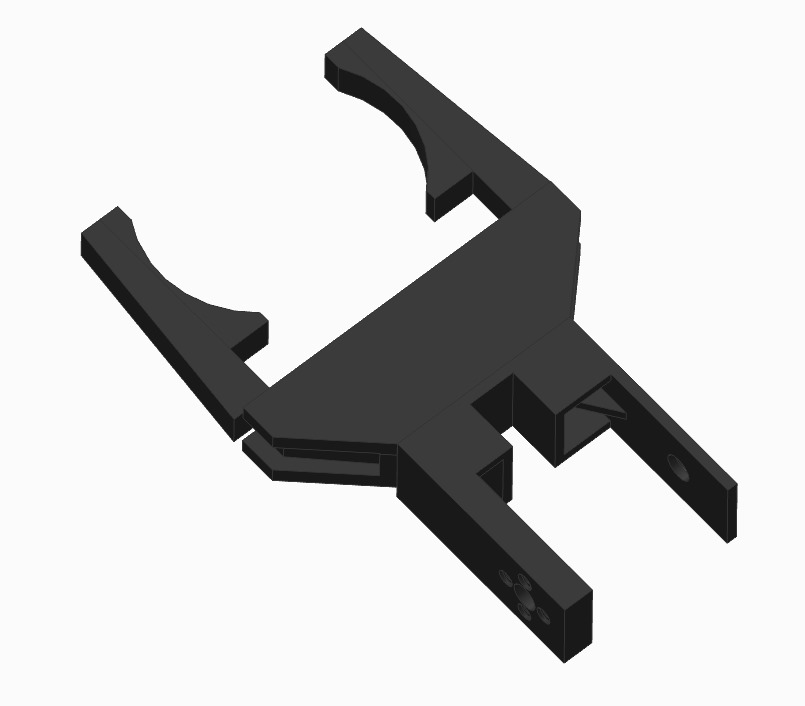
\includegraphics[width=0.7\textwidth]{img/pinza_tapa.png}
        \caption{Vista del gripper ensamblado mostrando la configuración de mordazas paralelas y carcasa de protección.}
        \label{fig:gripper_Real}
    \end{subfigure}
    \caption{Efector final tipo gripper con transmisión por piñón-cremallera para agarre adaptativo de lechugas.}
\end{figure}

\paragraph{Consideraciones de diseño para manipulación de cultivos}

El agarre de lechugas presenta desafíos particulares debido a la estructura delicada y heterogénea de las hojas. El diseño implementa las siguientes soluciones:

\begin{itemize}
    \item Mordazas con geometría envolvente que distribuyen la fuerza de agarre sobre mayor superficie de contacto
    \item Control de fuerza máxima mediante limitación de torque del servomotor
    \item Superficies de contacto texturizadas que incrementan fricción sin elementos penetrantes
    \item Velocidad de cierre controlada para evitar impactos bruscos
\end{itemize}

La combinación de estos elementos permite tasas de agarre exitoso superiores al 80\% en pruebas con lechugas de diferentes tamaños y configuraciones de hojas, como se detalla en la sección de pruebas experimentales del presente informe.
